\chapter{The GCWizard - contribute with new features}

\section{Providing Symbol tables}
If you want to provide your favorite symbol tables you have two options:
\begin{itemize}
    \item you can send the symbols via E-Mail
    \item you can provide the symbols via git
\end{itemize}
However, there are some commonalities to consider.

\subsection{Commonalities}
\begin{description}
    \item [Style guide] \,
    \begin{itemize}
        \item A Symbol-set consists of several pictures: One picture per symbol. So if a symbol table shows 26 symbols for 26 letters, you have to send these 26 symbols as single pictures.
        \item Please make sure that the symbols are aligned more or less evenly so that they appear ordered in the overall view afterwards: not one symbol sticks to the right edge and the next one on top, etc.
        \item The picture sizes are 150×150 pixels in the best case. If the original source does not provide this resolution, there is of course nothing you can do.
        \item The pictures are saved as PNG-file
        \item It would be nice if the pictures had a transparent background. This will make it easier to change the design later on, where the symbols might need to be set onto a different color. However, this is not planned at the moment. Therefore it is also not a big disadvantage if you deliver the symbol images with a white background. Graphically inexperienced people often have difficulties with this step and shy away from the whole work. So don’t be put off by this, this is a Nice-To-Have
    \end{itemize}
    \item [The File Names of the symbol files] \,
    \begin{itemize}
        \item Basically, it is simple: The images should have the ASCII code of the displayed character. So if a symbol shows the letter A, the picture is called 65.png because the ASCII value of A is 65. The background is that the GCWizard builds the symbol tables essentially completely automatically. Basically, the new image sets are registered in the program and the GCWizard reads the necessary information from the file names and thus builds the tables. It is now possible that a symbol shows an exclamation mark, for example. But if the file names would be called A.png instead of 65.png, we would have a problem with the exclamation mark, because the file name !.png is not allowed. With the ASCII value we are much more flexible.
        \item If a symbol encodes several characters, e.g. the same symbol is used for both, A and 1, the symbol is saved twice, e.g. as 65.png for \enquote{A} and once again as 49.png for \enquote{1.}
        \item It can also happen that there are two symbols for the same character; i.e. two different pictures show a space. Then we would have the file 32.png twice, which leads to problems. In this case, an underscore is simply appended to the second file. So we gain the files 32.png and 32\_.png
        \item Special cases: There are symbols that encode more than one character (e.g. “SCH”, “CH”, “NG”) or even entire commands (e.g. “START”, “ERROR”, “CANCEL”). These are special cases that (currently) have to be handled manually during maintenance. These files are then simply called like this: sch.png or start.png
        \item Upper/lower case: In general, symbol tables are not case sensitive. In this case, the files should be upper case (ASCII values 65 to 90). However, there are some cases where there are different symbols for upper and lower case letters. In this case, the file should be named accordingly (i.e. add ASCII values from 97 to 122 for lower case letters). It would be great if you would point this out on delivery, so that we can take it into account when entering the data.
    \end{itemize}
    \item [Sources for the pictures] \,
        \begin{itemize}
            \item The sources for the symbols should be freely available or there must be an explicit permission to use these symbols. The best source is Wikipedia or its media repository, the Wikimedia Commons. We also have permission to use the old myGEOtools tables. There are certainly a number of other possible sources like for example pinterest: \url{https://www.pinterest.de/silke161066/geocaching-codetabellen/}.   
            \item NO source is kryptografie.de, where we have unfortunately received an explicit refusal of cooperation!
        \end{itemize}
    \item [The workflow for creation] \,\\
         Basically it is completely up to you how and with which graphic tool (GIMP, Photoshop, CorelDraw or just Paint) you do all this. There are endless tools and even more ways to achieve all this. I provide here the manual that Äggsbärde created in the German geoclub.de forum and which describes his own workflow:
        \begin{itemize}
            \item Open the PDF page of geotools in the graphics program of your choice.
            \item Mark the background with the “magic wand” tool (you may have to play with the slider to make sure it doesn’t mark too much or too little).
            \item Eventually rework selection with selection tool and then remove the background.
            \item Now it is a transparent background.
            \item Now cut out the largest character/symbol with the Selection tool.
            \item Create a new file.
            \item When creating, the \enquote{dimensions} of the image are taken directly from the clipboard. I create the new image rectangular and with a few pixel offset bigger.
            \item Now the remaining symbols are cut out and pasted as a layer into the new file and aligned.
            \item Cut the whole file again if necessary (too much empty margin) and then reduce/enlarge it to 150×150 pixels.
            \item At the end save the individual layers as PNG under the ASCII code.
        \end{itemize}
\end{description}

\subsection{Contribute via E-Mail}
Finally, put all symbols into an archive file of your choice e.\,g. zip, 7z, rar, \dots and send it to Mark: \url{geocache.wizard@gmail.com}.

\subsection{Contribute via git}
If you are familiar with git and its concepts you can also download the GCWizad source-code, create a feature branch with the directories for your symbol sets and finally create a Pull request.

Your Symbol-sets with the corresponding directories should be sub-directories of \emph{\textbackslash assets\textbackslash symbol\_tables}.\par

Details about working with git are found in chapter \ref{chapter-git}. 

\section{Providing new tools for Encodings and decodings, Scientific and technology or games}
The most challenging part is the contribution with new features. Therefore working with git is the prerquisite. As an example for this step-by-step-tutorial we will create a feature which increases and decreases a given number.

\subsection{Building the Backend -- Logic}
The business logic is located in \emph{\textbackslash lib\textbackslash logic}. For crypto tools you should choose the path \emph{\textbackslash lib\textbackslash logic\textbackslash tools\textbackslash crypto\_and\_encodings}.\par 

Create a well-named new dart file. Assuming, your encrypting algorithm is called \enquote{Increased N}, you should call your file \emph{increased\_n.dart}, everything in lower case, using underscores. If you are planning a more difficult feature with some sub function, think about a sub directory e.g. as the coordinate functions or the math/primes functions. \par

Dart coding guidlines recommend not creating a class if you only want to write static functions, as we will. You need a static function for each, encryption and decryption. The entry functions, which will be called later by external methods or the widget, should be called \emph{encryptX/decryptX} or, in case of encodings, \emph{encodeX/decodeX}. Please ensure, that you catch some edge cases and return either null or an empty string or whatever fits in that case:

\begin{lstlisting}
encryptIncreasedN(int number) {
  if (number == null)
    return null;

  return number + 1;
}

decryptIncreasedN(int number) {
  if (number == null)
    return null;

  return number - 1;
}
\end{lstlisting}
\captionof{lstlisting}{Logic-Example IncreaseN}
\label{fig: logic}

\subsection{Building the Frontend -- Widget}
In Flutter, everything is a widget. Widgets are just tiny chunks of UI that you can combine to make a complete app. Building an app Flutter is like building a lego set — piece by piece.
Widgets are nested inside of each other to build your app. Even the root of your app is just a widget. It’s widgets all the way down.
The most important part of using Flutter Widgets effectively is designing your lowest level widgets to be reusable.\par
\bigskip
%
Widget classes have (usually) only one requirement: it must have a build method which returns other Widgets. The only exception to this rule is low-level widgets like \emph{Text} that return primitive types like Strings or numbers, usually.
Flutter widgets must extend a handful of classes from the Flutter library. The two you’ll use almost always are \emph{StatelessWidget} and \emph{StatefulWidget}.\\
The difference is that one has a concept of state within the Widget and some built in methods that tells Flutter to re-render if that state changes. This is a key concept in Flutter. Hence StatefulWidget has two classes: the state object and the widget.\par
\bigskip
%
The GCWizard-Widgets are located in \emph{/lib/widgets/}. The sub directory, again, follows the structure of the logic directory. That means your widget should be located into \emph{/lib/widgets/tools/crypto\_and\_encodings/increased\_n.dart}.\par
\bigskip
%
The widget structure supports you by encapsuling the boiler plate code for the simple widget creation, the navigation to the widget, the scrolling, the title and so on. You simply have to write a layout for inputs and outputs. All widgets are of type \emph{StatefulWidget}, their state management -- if you like, their whole frontend logic -- is in their State-class. The most important one is the build()-method in the state class, which will be called by the framework to build your frontend.\par
\bigskip
%
Usually -- as long as no-one has a better idea -- you will return a Column()-widget, which layouts your input fields and output fields and everything else in vertically order.

\begin{figure}[H]
    \centering
    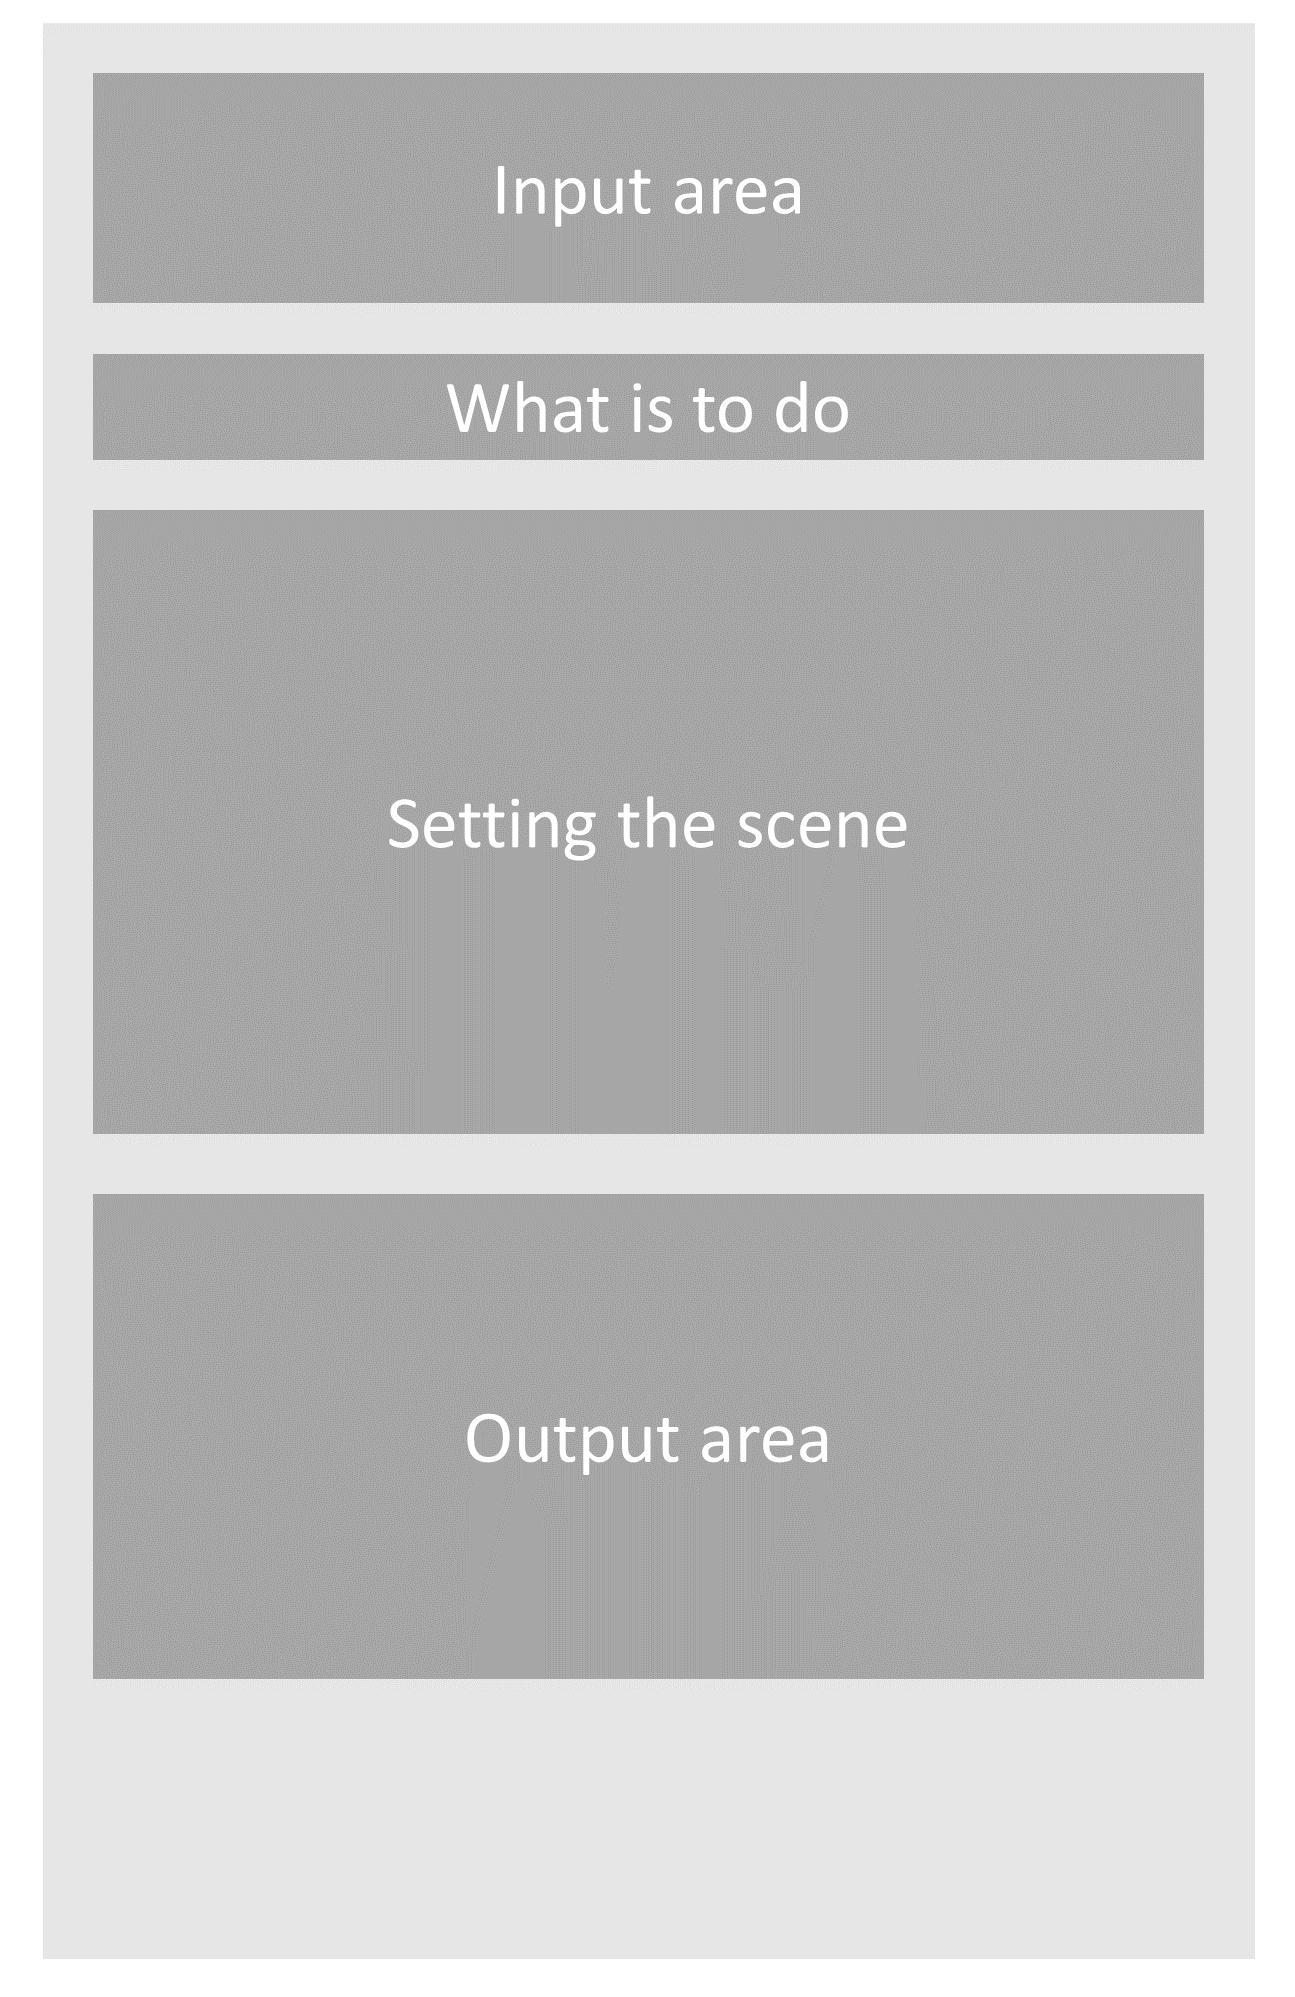
\includegraphics[width=0.7\linewidth]{Bilder/layout-high-level}
    \caption{Layout areas}
    \label{fig:layout-high-level}
\end{figure}
 
It's very important that you always import the widgets from the \emph{material.dart} and not the \emph{cupertino.dart}, which mostly contains the same widgets, but which is only for iOS.\par

This could be your stub, which would show an empty page with title:

\begin{lstlisting}
import 'package:flutter/material.dart';

class IncreasedN extends StatefulWidget {
  @override
  IncreasedNState createState() => IncreasedNState();
}

class IncreasedNState extends State<IncreasedN> {

  @override
  Widget build(BuildContext context) {
    return Column(
             children: <Widget>[

             ],
           );
  }
}
\end{lstlisting}
\captionof{lstlisting}{Widget-Example IncreaseN -- Basic Structure}
\label{fig: widgetstructure}

\subsubsection{Create the structure}
For this example you need a integer-text field and a switch for encrypt/decrypt. Furthermore you need an output field.

\paragraph{Integer TextField} There are already many specialized widgets. You can find them in the \emph{widgets/common/-directory}. So, of course, there is already a special TextField for integer inputs, which:
\begin{itemize}
    \item already has an input controller,
    \item allows only digits inputs,
    \item returns both, the real entered text and the parsed integer input.
\end{itemize}

It is called \emph{GCWIntegerTextField}, which we take for simplicity. But, for real cases, there is another widget, which fits better: The \emph{GCWIntegerSpinner}, which adds +/- buttons next to the TextField. A complete list of all predefined Widgets are part of the annex.

\paragraph{The mode switch} There are two types of switches: The first is a simple on/off switch, which returns \emph{true} and \emph{false}, and a two-options switch, which returns the switch position \emph{left} or \emph{right}. Without any further configuration, it already shows: \emph{Mode: Encrypt/Decrypt}. This is called \emph{GCWTwoOptionsSwitch}.

\paragraph{The output} Of course, there is already a widget for it. It paints a divider with localized Output-text and it provides a formatted Text widget for the content. You only have to put the text to it. It's name is \emph{GCWOutputText}. 

\begin{lstlisting}
import 'package:flutter/material.dart';
import 'package:gc_wizard/widgets/common/base/gcw_output_text.dart';
import 'package:gc_wizard/widgets/common/gcw_integer_textfield.dart';
import 'package:gc_wizard/widgets/common/gcw_twooptions_switch.dart';
import 'package:gc_wizard/logic/tools/crypto_and_encodings/increased_n.dart';

class IncreasedN extends StatefulWidget {
  @override
  IncreasedNState createState() => IncreasedNState();
}

class IncreasedNState extends State<IncreasedN> {
    
  @override
  Widget build(BuildContext context) {
    return Column(
             children: <Widget>[
               GCWIntegerTextField(),  // here are your widgets
               GCWTwoOptionsSwitch(),
               GCWOutputText(
                 text: //TODO
               )
             ],
           );
  }
}
\end{lstlisting}
\captionof{lstlisting}{Widget-Example IncreaseN -- Basic Layout}
\label{fig: widgetlayout}

\subsubsection{Store the values and calculate the output}
Every widget returns a value: The integer input returns an integer and the switch returns its position. On the other hand, the output text presumes the output text.\par 

So, you have to create some local variables to store the input values and to hand over the result to the output. Also you need an event, where you can get or set the data. Most widgets can take a function callback for their \enquote{onChanged-events}. This is the point to receive the values

\begin{lstlisting}
class IncreasedNState extends State<IncreasedN> {
    
    //define local variables and initialize them
    
    var _currentIntegerValue = {'text': '', 'value': 0}; 
    // this is how the return value of the GCWIntegerTextField looks like. 
    // There is a global variable for the initial value: defaultIntegerText
    
    var _currentMode = GCWSwitchPosition.left;
    
    @override
    Widget build(BuildContext context) {
        return Column(
        children: <Widget>[
        GCWIntegerTextField(
        onChanged: (ret) {              // onChanged callback for TextField
            setState(() {
                _currentIntegerValue = ret; // set value
            });
        }
        ),
        GCWTwoOptionsSwitch(
        onChanged: (value) {            // onChanged callback for Switch
            setState(() {
                _currentMode = value;   // set value
            });
        },
        ),
        GCWOutputText(
        text: //TODO
        )
        ],
        );
    }
}
\end{lstlisting}
\captionof{lstlisting}{Widget-Example IncreaseN -- Get input}
\label{fig: widgetinput}

\subsubsection{Calculate and set output}
There are several ways to do it. You surely noticed the \emph{setState()-calls} in the \emph{onChanged()-callbacks}. They trigger a widget rebuild. So, in that case, everytime a value has changed, the widget will be rebuild. And the output will be recalculated. So, you can add the calculation directly to the text attribute of the \emph{GCWOutputText}. Because, usually your layout would be much more complex, so, it is better to extract this calculation to a method, which should return a string in all cases:

\begin{lstlisting}
class IncreasedNState extends State<IncreasedN> {
    
    var _currentIntegerValue = defaultIntegerText; // here the global variable is used
    var _currentMode = GCWSwitchPosition.left;
    
    @override
    Widget build(BuildContext context) {
        return Column(
        children: <Widget>[
        GCWIntegerTextField(
        ...
        ),
        GCWTwoOptionsSwitch(
        ...
        ),
        GCWOutputText(
        text: _buildOutput()            // call the ouput method
        )
        ],
        );
    }
    
    _buildOutput() {
        if (_currentIntegerValue == null) // catch some edge cases
        return '';
        
        var calculated = _currentMode == GCWSwitchPosition.left
        ? encryptIncreasedN(_currentIntegerValue['value'])  // Position.left == encrypt; 
        // notice the ['value'] part, which takes the parsed integer value from the text field result
        : decryptIncreasedN(_currentIntegerValue['value']); // Position.right == decrypt
        
        return calculated == null ? '' : calculated.toString();
    }
}
\end{lstlisting}
\captionof{lstlisting}{Widget-Example IncreaseN -- Set output}
\label{fig: widgetoutput}


\subsection{Internationalization}
In the directory \emph{/assets/i18n/} you can find all language files. These are key/value JSON files, each for every supported language. You already used a localization key in the registry, which is mapped here to the title, the description- and an example-title is neccessary, others are optional but recommended. This needs to be transferred to a real text. So, please add all used keys -- maybe you used some directly in your widget as well -- and put the text in the specific language:

\begin{lstlisting}
"increasedn_title" : "Increased N",
"increasedn_description" : "Increases an integer value by 1",
"increasedn_example" : "41 $\Rightarrow$ 42",
\end{lstlisting}
\captionof{lstlisting}{den.json}
\label{fig: json-en}

\begin{lstlisting}
"increasedn_title" : "Inkrementiertes N",
"increasedn_description" : "Erhöht eine Ganzzahl um 1",
"increasedn_example" : "41 $\Rightarrow$ 42",
\end{lstlisting}
\captionof{lstlisting}{de.json}
\label{fig: json-de}

\subsection{Registration of the feature}
All widgets are registered centrally. The file is \emph{/widgets/registry.dart}. This imports your widget, wraps your layout with a real page widget, adds a keyword for the language files which will be mapped to title, description and example, the category, where the tool fits -- usually \emph{CRYPTOGRAPHY} for codes or \emph{SCIENCE\_AND\_TECHNOLOGY} for some scientific formula stuff and even the keywords for the search engine without umlauts or diacritics:

\begin{lstlisting}
import 'package:gc_wizard/widgets/tools/crypto_and_encodings/increasedn.dart';
...
  GCWToolWidget(
    tool: IncreasedN(), 
    i18nPrefix: 'increasedn', 
    category: ToolCategory.CRYPTOGRAPHY,
    searchStrings: 'increasedn'
  ),
...
\end{lstlisting}
\captionof{lstlisting}{Example registry.dart for IncreaseN}
\label{fig: registry}

Notice, that the toolname is a call of the \emph{i18n()-method}. This is for internationalization. It maps the given keyword \emph{increasedn\_title} in this case to the real output in all available languages. \par
\bigskip
Finally, the the widget has to be put into a list. This means: Every widget has a list as parent. Most widget are located in the main list, which is shown on the main screen. But some tools, like the coordinate functions are part of an own list. 
All lists order their tools by their localized titles. \\
So, this tool can be put into the main list, which can be found in \emph{/widgets/main\_view.dart}, around lines 112ff\dots Add line and import of the widget-file:

\begin{lstlisting}
import 'package:gc_wizard/widgets/tools/crypto_and_encodings/increased.dart';
...
className(IncreasedN()),
...
...
\end{lstlisting}
\captionof{lstlisting}{Example main\_view.dart for IncreaseN}
\label{fig: mainview}


\subsection{Building tests}
Tests for the logic are essential: First, they ensure that the logic works as expected and they ensure, that a possible change will not destroy the current functionality. Second, they serve as a documentation. If somebody wants to know, how a certain functions works, he or she can take a look at the test cases, check out the parameters and can see the expected result. This is also one of the first things, a reviewer for Pull Requests checks out before he or she will take a look at the real code.\par
\bigskip
Tests are located in the \textbackslash test-directory. Its structure follows the main structure. \newline
So, your test should be located into \emph{\textbackslash test\textbackslash logic\textbackslash tools\textbackslash crypto\_and\_encodings\textbackslash increased\_n.dart}.

\subsubsection{Test structure}
There are test groups. Every group is for testing a specific method. Usually there are two groups, one for encryption/encoding and one for decryption/decoding. Every group gets a list of input values, combined with the specific expected output.  Every list entry is a key/pair map, which should mirror the parameter names and their values. Afterwards this list will be iterated. For every list entry the relevant function will be called. Please add some well-thought test cases, some crazy values and, of course, the typical cases \enquote{null} and, if relevant, empty strings or lists.


\begin{lstlisting}
import 'package:flutter_test/flutter_test.dart';
import 'package:gc_wizard/logic/tools/crypto_and_encodings/increased_n.dart';

void main() {
  group('IncreasedN.encrypt:', () {
    List<Map<String, dynamic>> _inputsToExpected = [
      {'number' : null, 'expectedOutput' : null},
      {'number' : -42, 'expectedOutput' : -41},
      {'number' : -1, 'expectedOutput' : 0},
      {'number' : 0, 'expectedOutput' : 1},
      {'number' : 1, 'expectedOutput' : 2},
      {'number' : 42, 'expectedOutput' : 43},
    ];

    _inputsToExpected.forEach((elem) {
      test('number: ${elem['number']}', () {
        var _actual = encryptIncreasedN(elem['number']);
        expect(_actual, elem['expectedOutput']);
      });
    });
  });

  group('IncreasedN.decrypt:', () {
    List<Map<String, dynamic>> _inputsToExpected = [
      {'number' : null, 'expectedOutput' : null},
      {'number' : -42, 'expectedOutput' : -43},
      {'number' : -1, 'expectedOutput' : -2},
      {'number' : 0, 'expectedOutput' : -1},
      {'number' : 1, 'expectedOutput' : 0},
      {'number' : 42, 'expectedOutput' : 41},
    ];

    _inputsToExpected.forEach((elem) {
      test('number: ${elem['number']}', () {
        var _actual = decryptIncreasedN(elem['number']);
        expect(_actual, elem['expectedOutput']);
      });
    });
  });
}
\end{lstlisting}
\captionof{lstlisting}{Testing-Example increaseN/decreaseN}
\label{fig: test}


